\documentclass[fleqn]{article}
\usepackage[UTF8]{ctex}
\usepackage{listings}
\usepackage{pdfpages}
\usepackage{color}
\usepackage[colorlinks,linkcolor=blue]{hyperref}
\usepackage{dashrule}
\usepackage{diagbox}
\usepackage[german]{babel}
\usepackage[T1]{fontenc}
\usepackage[latin1]{inputenc}
\usepackage{titlesec}
\usepackage{geometry}
\usepackage{qtree}
\usepackage{tikz}
\usepackage{amsmath}
\usepackage{amssymb}
\setcounter{secnumdepth}{0}
\usetikzlibrary{positioning}
\geometry{top=2.5cm, bottom=2.5cm}
\lstset{
 columns=fixed,       
 numbers=left,                                        % 在左侧显示行号
 numberstyle=\tiny\color{gray},                       % 设定行号格式
 frame=none,                                          % 不显示背景边框
 backgroundcolor=\color[RGB]{245,245,244},            % 设定背景颜色
 keywordstyle=\color[RGB]{40,40,255},                 % 设定关键字颜色
 numberstyle=\footnotesize\color{darkgray},           
 commentstyle=\it\color[RGB]{0,96,96},                % 设置代码注释的格式
 stringstyle=\rmfamily\slshape\color[RGB]{128,0,0},   % 设置字符串格式
 showstringspaces=false,                              % 不显示字符串中的空格
 language=c++,                                        % 设置语言
 breaklines,                                          % 自动换行
}

\title{DBG Zusammenfassung WS20/21}

% \author{Dongze Yang}

\begin{document}

\maketitle

\tableofcontents

\newpagestyle{main}{
    \sethead{}{}{DBG WS 20/21}
    \setfoot{}{\thepage}{}
    \headrule
    \footrule
}
\pagestyle{main}

\newpage

\section{UML - Unified Modeling Language 统一建模语言}

\subsection{Was ist UML}

\noindent $\circ$ Typ eines statischen Struktur-Diagrams 静态结构图的类型

\noindent $\circ$ beschreibt die Struktur eines Systems und zeigt 描述系统的结构并显示

> Klassen (Objekte / Entitäten) des Systems 系统的类(对象/实体)

> deren Attribute 他们的属性

> mögliche Operationen (oder Methoden) 可能的操作(或方法)

> Relationen (Beziehungen) zwischen den Klassen 类之间的关系

\noindent $\circ$ Verwendung im Datenbankdesign: 在数据库设计中使用

1. Hauptphase: Konzeptuelles DesignEntwicklung eines semantischen Datenmodells 主要阶段:概念设计,语义数据模型的开发

2. Hauptphase: Logisches DesignTransformation des konzeptuellen Modells in ein konkretes Datenmodell 主要阶段:逻辑设计,将概念模型转化为具体的数据模型

\subsection{UML - Beispiel}

\noindent\textbf{Bsp. 1}

\begin{center}
    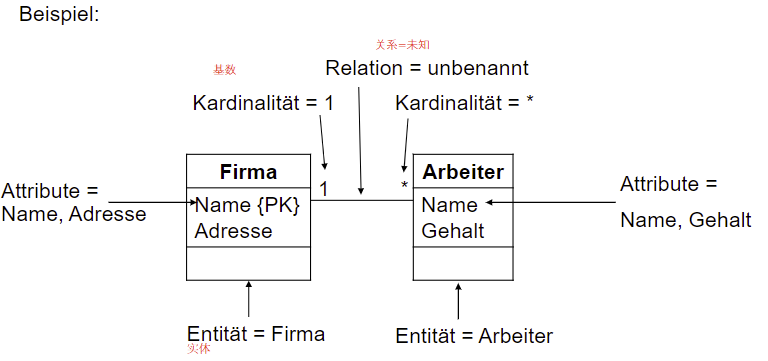
\includegraphics[scale=0.5]{1.png}
\end{center}  

\noindent---------------------------------------------------------------------------------------------------------------------------------

\noindent\textbf{Bsp. 2}

\begin{center} 
    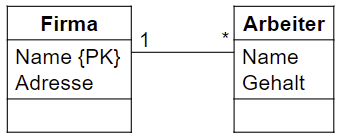
\includegraphics[scale=0.6]{2.png}
\end{center}

a)Keine zwei Firmen können den gleichen Namen haben. 两个公司不能有同样的名字($\checkmark$)

b)Keine zwei Arbeiter können den gleichen Namen haben. 两个员工不能用同样的名字($\times$)

c)Keine zwei Firmen können die gleiche Adresse haben. 两个公司不能有同样的地址($\times$)

d)Keine zwei Arbeiter können an der gleichen Adresse arbeiten. 两个员工不能用同样的地址($\times$)

e)Jeder Arbeiter arbeitet für mindestens eine Firma. 每个员工至少在一间公司工作($\checkmark$)

f)Kein Arbeiter arbeitet für mehr als eine Firma. 没有员工可以同时在多家公司工作($\checkmark$)

g)Jede Firma hat mindestens einen Arbeiter. 每个公司至少有一个员工($\times$)

h)Zwei gleichnamige Arbeiter können nicht für die gleiche Firma arbeiten. 两个同名员工不能在同一家公司工作($\times$)

i)Zwei gleichnamige Arbeiter können nicht für verschiedene Firmen arbeiten. 两个同名员工不能在不同公司工作($\times$)

\noindent---------------------------------------------------------------------------------------------------------------------------------

\noindent\textbf{Bsp. 3}

\begin{center} 
    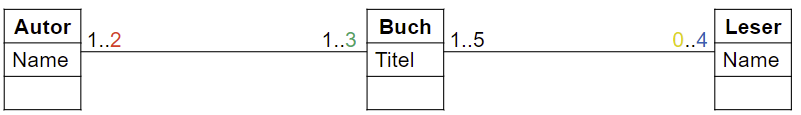
\includegraphics[scale=0.5]{3.png}
\end{center}

1 Buch可能有:1至2个Autor,0至4个Leser

1 Autor可能有:1至3本Buch

1 Leser可能读过:1至5本Buch

\noindent 若有6个Autor:

a) 最少/多有几本Buch? \qquad 最少:6/2*1=3, 最多:6*3=18

b) 最少/多有几个Leser? \qquad 最少:3*0 = 0, 最多:18*4=72

\noindent 若有6个Leser:

a) 最少/多有几本Buch? \qquad 最少:$\lceil 6/4 \rceil = 2$, 最多:6/0$\rightarrow\infty$

b) 最少/多有几个Autor? \qquad 最少:$\lceil 2/3 \rceil = 1$, 最多:$\infty * 2 \rightarrow\infty$

\subsection{Modelliere die Informationen in einem UML-D 在UML图中对信息进行建模}

\noindent\textbf{Bsp. 1}

有1个Online-Video-Verleih租赁服务,这个服务的Kunden有其ID和密码进行登录。他们可以租赁电影,每个电影有不同的名称和租金,但是只有当然他们有足够信誉Guthaben的情况下,才能观看。

\begin{center} 
    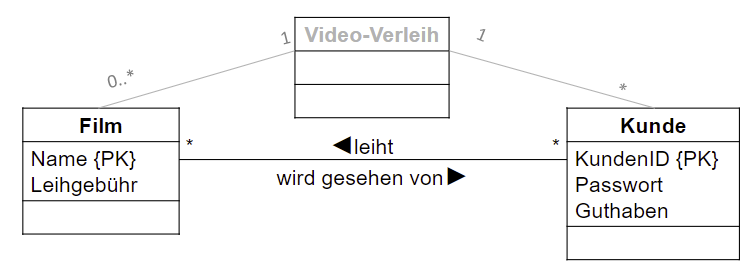
\includegraphics[scale=0.5]{4.png}
\end{center}

\subsection{UML Relationales Schema UML关系方案}

\noindent Relationales Schema für Datenbanken Grundlagen in vereinfachter Form 数据库的关系模式

\noindent Jede neue Zeile bildet ein Schema für jede Entität 每条新行形成每个实体的架构

\noindent Attribute werden in Klammern dahinter geschrieben 属性写在方括号后面

\noindent Primärschlüssel (PK) wird unterstrichen PK主键带下划线

\noindent Fremdschlüssel(FK) wird markiert FK外键加粗
\\
\\
\noindent Relationales Schema Übertrag: 关系架构结转:

-jede Entität verlangt eigenes Schema mit PK 每个实体都需要自己的PK方案

-1 zu 1: einfaches Schema mit FK 1对1:使用FK的简单方案

-1 zu * ohne Beschreibung: FK auf * Seite im Schema 1对*无说明:方案中FK在*页

-1 zu * mit Beschreibung: Beschreibung verlangt FK ODER eigenes Schema mit PK und FK 1对*带说明:说明需要FK或他自己带有PK和FK的方案

-* zu *: Eigenes Schema mit PK und FK *对*:具有PK和FK的方案。

\begin{center} 
    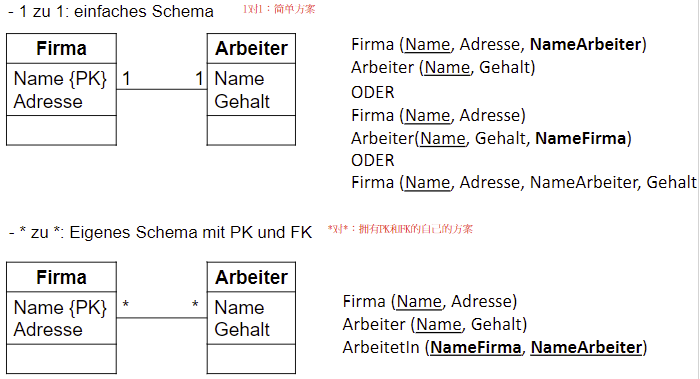
\includegraphics[scale=0.5]{5.png}
    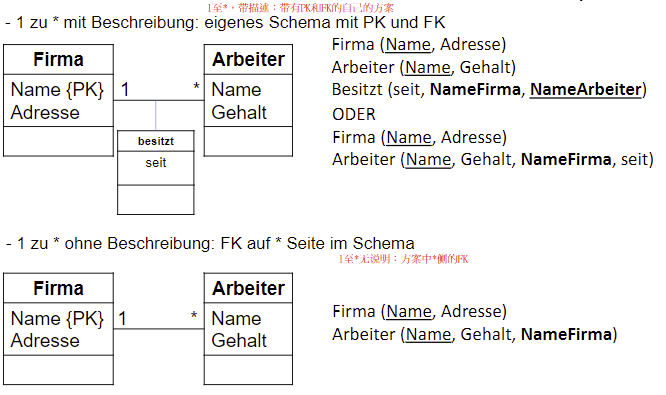
\includegraphics[scale=0.5]{6.png}
\end{center}

\subsection{UML关系方案建模 Beispiel}

\noindent\textbf{更多见Übung 3, 4}

\noindent\textbf{Bep. 1}

在办公室Büroräumen(zinr)中,自一个时间点Zeitpunkt(seit)有员工Mitarbeiter(persnr,name,titel,status)在一个确定的位置Platz(platz)。在房间里有电话Telefone(telnr),这个电话可能连接到Hausapparat或Amtsapparat(art)。

\begin{center} 
    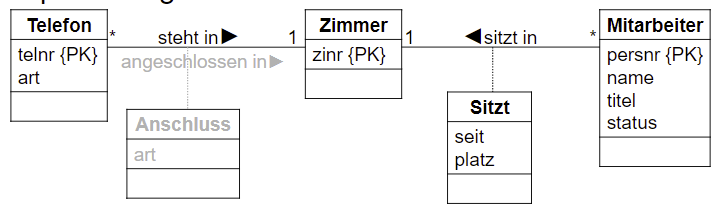
\includegraphics[scale=0.5]{7.png}
\end{center}

\noindent relationale Schema:

Zimmer(\underline{zinr})

Mitarbeiter(\underline{persnr},name,titel,status)

Sitzt(seit,platz,\underline{\textbf{persnr}},\textbf{zinr})

Telefon(\underline{telnr},art,\textbf{zinr})

\noindent---------------------------------------------------------------------------------------------------------------------------------

\noindent\textbf{Bep. 2}

一个Büromöbelfirma卖家具Möbel(moe\_nr, bez, preis),

这些家具由不同的供应商Zulieferbetrieben(zulief\_nr, bez, adresse)订做Spezialanfertigungen(Furnier),

这就是为什么交货时间Lieferzeiten(lieferzeit)不同的原因。

每件家具可以有不同的贴面Furnieren(farb\_nr, bez)制成。

在公司中有员工Angestellte(pers\_nr,name,geb\_dat, seit, gehalt)

与顾客Kunden(kd\_nr, name, adresse)

签订合同Kaufverträge(vertr\_nr, bestell\_dat),

每个合同中包括相应Ausfertigung(Furnier)的多个家具件Möbelstücken(anz)。

在交货后每个合同都要签订一份账单Rechnung(rech\_nr, lief\_dat, preis, bezahlt)。

\begin{center} 
    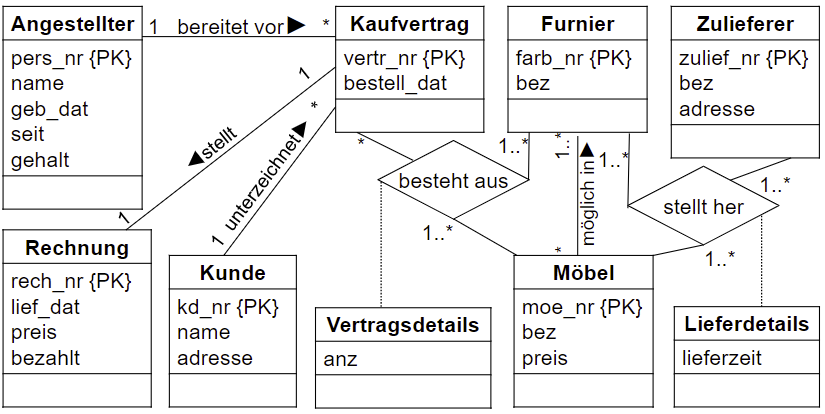
\includegraphics[scale=0.5]{18.png}
\end{center}

\noindent relationale Schema:

Angestellter (\underline{pers\_nr}, name, geb\_dat, seit, gehalt)

Kunde (\underline{kd\_nr}, name, adresse)

Kaufvertrag (\underline{vertr\_nr}, bestell\_dat, \textbf{kd\_nr}, \textbf{pers\_nr})

Rechnung (\underline{rech\_nr}, lief\_dat, preis, bezahlt, \textbf{vertr\_nr})

Möbel (\underline{moe\_nr}, bez, preis)

Furnier (\underline{farb\_nr}, bez)

Zulieferer (\underline{zulief\_nr}, bez, adresse)

Möbelfarbe (\underline{\textbf{moe\_nr}}, \underline{\textbf{farb\_nr}})

Vertragsdetails (\underline{\textbf{moe\_nr}}, \underline{\textbf{farb\_nr}}, \underline{\textbf{vertr\_nr}}, anz)

Lieferdetails (\underline{\textbf{moe\_nr}}, \underline{\textbf{farb\_nr}}, \underline{\textbf{zulief\_nr}}, lieferzeit)

\subsection{häufige UML-Fehler}

\noindent\textbf{Bep. 1}

\begin{center} 
    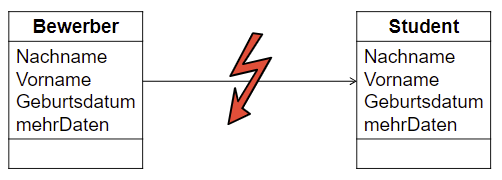
\includegraphics[scale=0.5]{8.png}
\end{center}

Wenn nach Zulassung ein Datensatz von ,,Bewerber'' zu ,,Student'' kopiert wird (eventuell mit Überarbeitung), fügen wir deshalb KEINE assoziative Verbindung zwischen Bewerber und Student ein, da es sich um den Kontrollfluss handelt.

若两个类一致,并要将其中一个类的数据复制到另一个中,他们之间不建立关系。

\noindent---------------------------------------------------------------------------------------------------------------------------------

\noindent\textbf{Bep. 2}

\begin{center} 
    
\includegraphics[scale=0.5]{9.png}
\end{center}

关系名称重复,对于同一个类上的关系应具有唯一名称。Alle Relationen sollten eindeutige Namen haben.

Attribute verschiedener Entitäten dürfen hingegen gleich sein. 但不同实体的属性可能相同。

\begin{center} 
    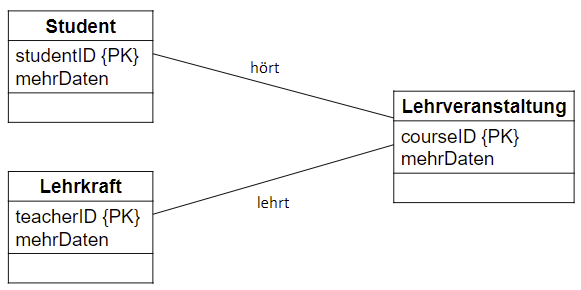
\includegraphics[scale=0.5]{10.png}
\end{center}

\noindent---------------------------------------------------------------------------------------------------------------------------------

\noindent\textbf{Bep. 3}

\begin{center} 
    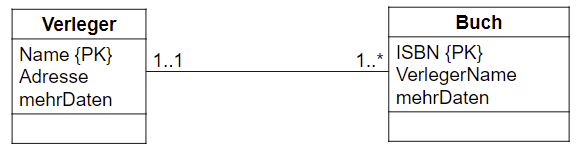
\includegraphics[scale=0.5]{11.png}
\end{center}

Vermeide implizite Assoziationen 避免隐式关联

der Name des Verlegers ist eine implizite Assoziation, welche redundant ist. Verleger的Name是一个隐式关联,这是多余的。

$\rightarrow$ durch die Relation/Verbindung hat jedes Buch bereits einen Verleger mit diversen Attributen.
由于这种关系/联系,每本Buch已经有一个具有各种属性的Verleger了。

\begin{center} 
    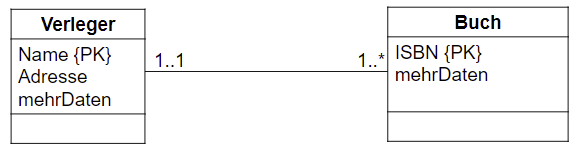
\includegraphics[scale=0.5]{12.png}
\end{center}

\noindent---------------------------------------------------------------------------------------------------------------------------------

\noindent\textbf{Bep. 4}

\begin{center} 
    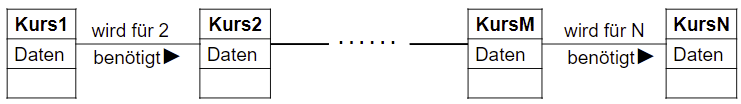
\includegraphics[scale=0.5]{13.png}
\end{center}

UML ist immer genau definiert UML图始终是精确定义的

Rekursive Vorschriften habe eine andere Notation 递归规则有不同的表示法。

keine Platzhalter in UML-Diagrammen. UML图中没有占位符。

\begin{center} 
    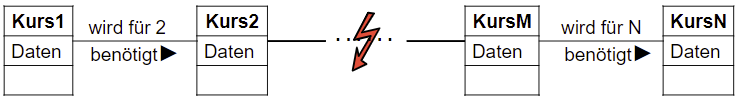
\includegraphics[scale=0.5]{14.png}
\end{center}

Rekursive表示法:

UML-Diagramme haben eine genau definierte Anzahl von Entitäten und Relationen. UML图具有精确定义的实体数和关系数。

\begin{center} 
    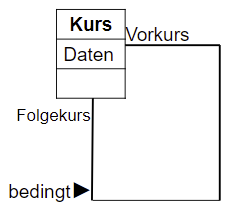
\includegraphics[scale=0.5]{15.png}
\end{center}

\noindent---------------------------------------------------------------------------------------------------------------------------------

\noindent\textbf{Bep. 5}

\begin{center} 
    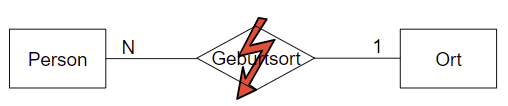
\includegraphics[scale=0.5]{16.png}
\end{center}

verwende UML und nicht Chens Notation für ERDs. 使用UML而不是Chens符号。

Peter Chen hat 1976 die nach ihm benannte Notation eingeführt, welche jahrelang für die Entity-Relationship-Modellierung in Form von Entity-Relationship-Diagrammen verwendet wurde.

\begin{center} 
    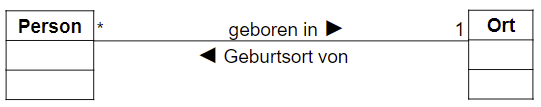
\includegraphics[scale=0.5]{17.png}
\end{center}

\section{Relationale Algebra 关系代数}

\subsection{定义}

Wir erzeugen Relationen aus anderen Relationen. 我们从其他关系中创造关系。

Die relationale Algebra kennt Rechen Operatoren und JoinOperationen. 关系代数识别为算术运算和连接运算。
\\
\\
6 Grundrechen \textbf{Operatoren} der Relationalen Algebra: 6种关系代数的基本算数运算:

\noindent \textbf{-Selektion} : $\sigma$ = Tupel werden nach Operator selektiert 

jedes Tupel wird nach BOOL geprüft

z.B. $\sigma$Gehalt>5000(Mitarbeiter) = Tupel mit BOOL=true

\noindent \textbf{-Projektion} : $\pi$ = wählt Teilmenge der Relation aus

R' ist Teilmenge von R1 als Tupel

z.B. $\pi$Gehalt(Mitarbeiter) = ganze Spalte Gehalt

\noindent \textbf{-Vereinigung} : $\cup$= zwei Relationen werden zu R'

Bedingung: Eingabeschema muss identisch sein

z.B. R'=Mitarbeiter $\cup$ Fotographen

\noindent \textbf{-Differenz} : -oder /= eine Relation wird von der anderen Relation abgezogen

Bedingung: Eingabeschema muss identisch sein

z.B. R'= Mitarbeiter -Fotographen

\noindent \textbf{-Kreuzprodukt} : $\times$= zwei Relationen werden mit allen Attributen zusammengefügt

Jedes Tupel von R1 wird mit jedem Tupel von R2 verbunden

z.B. R' = Mitarbeiter $\times$ Gehälter

\noindent \textbf{-Umbenennung} : $\rho$= Umbenennung von Relationen oder Attributen

z.B. Attribut $\rho$(Lohn<-Gehalt(Mitarbeiter))

z.B. Relation $\rho$(Angestellte'(Mitarbeiter))

\noindent---------------------------------------------------------------------------------------------------------------------------------

\noindent \textbf{-Selektion 选择} : $\sigma$ = 根据运算符选择元组 

根据BOOL检查每个元组

z.B. $\sigma$Gehalt>5000(Mitarbeiter) = Tupel mit BOOL=true

\noindent \textbf{-Projektion 投影} : $\pi$ = 选择关系R的子集

R'是R1的子集,作为元组

z.B. $\pi$Gehalt(Mitarbeiter) = ganze Spalte Gehalt 整列薪水

\noindent \textbf{-Vereinigung 联合} : $\cup$= 两个关系合并为R'

条件:输入方案必须相同

z.B. R'=Mitarbeiter $\cup$ Fotographen

\noindent \textbf{-Differenz 差} : '-' 或 '/' = 将一个关系从另一个关系中移除

条件:输入方案必须相同

z.B. R'= Mitarbeiter - Fotographen

\noindent \textbf{-Kreuzprodukt 叉积} : $\times$= 两个关系用所有属性组合在一起

R1的每个元组与R2的每个元组相连

z.B. R' = Mitarbeiter $\times$ Gehälter

\noindent \textbf{-Umbenennung 重命名} : $\rho$= 关系或属性的重命名

z.B. Attribut $\rho$(Lohn<-Gehalt(Mitarbeiter))

z.B. Relation $\rho$(Angestellte'(Mitarbeiter))

\begin{center}
    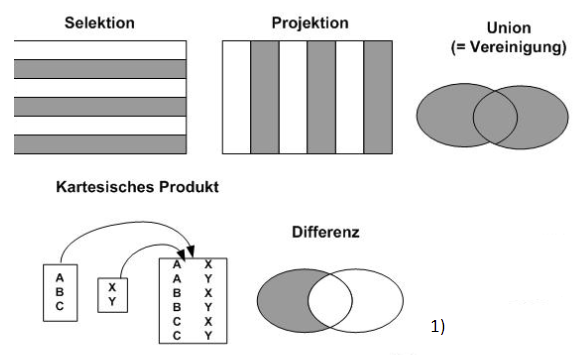
\includegraphics[scale=0.5]{19.png}
\end{center}

\noindent---------------------------------------------------------------------------------------------------------------------------------

\subsection{Beispiel}

\noindent\textbf{Bsp. 1}

已知关系R1, R2, R3。

\begin{center}
    R1=\begin{tabular}{|c|c|}
        \hline
        A1&A2\\
        \hline
        a&2\\
        b&2\\
        c&3\\
        \hline
    \end{tabular}
    R2=\begin{tabular}{|c|c|}
        \hline
        B1&B2\\
        \hline
        a&2\\
        d&4\\
        \hline
    \end{tabular}
    R3=\begin{tabular}{|c|}
        \hline
        C1\\
        \hline
    \end{tabular}
\end{center}

Erstelle dazu die \textbf{Ergebnisrelationen} für folgende Operationen 
und bestimme jeweils \textbf{den Grad des Ergebnisrelations-schemas} sowie 
\textbf{die Kardinalität der Ergebnisrelation}.

请为以下操作创建结果关系,并确定关系模式的程度以及结果关系的基数。

a)$\sigma$[A2 = 2] (R1)

\begin{center}
    R'=\begin{tabular}{|c|c|}
        \hline
        A1&A2\\
        \hline
        a&2\\
        b&2\\
        \hline
    \end{tabular}

    G: 2, K= 2.
\end{center}

b)$\pi$[A2] (R1)

\begin{center}
    R'=\begin{tabular}{|c|}
        \hline
        A2\\
        \hline
        2\\
        3\\
        \hline
    \end{tabular}

    G: 1, K= 2.
\end{center}

c)R1 $\cup$ R2

\begin{center}
    R'=\begin{tabular}{|c|c|}
        \hline
        A1&A2\\
        \hline
        a&2\\
        b&2\\
        c&3\\
        d&4\\
        \hline
    \end{tabular}

    G: 2, K: 4.
\end{center}

d)R1 - R2

\begin{center}
    R'=\begin{tabular}{|c|c|}
        \hline
        A1&A2\\
        \hline
        b&2\\
        c&3\\
        \hline
    \end{tabular}

    G: 2, K: 2.
\end{center}

e)R1 $\times$ R2

\begin{center}
    R'=\begin{tabular}{|c|c|c|c|}
        \hline
        A1&A2&B1&B2\\
        \hline
        a&2&a&2\\
        a&2&d&4\\
        b&2&a&2\\
        b&2&d&4\\
        c&3&a&2\\
        c&3&d&4\\
        \hline
    \end{tabular}

    G: 4, K: 6.
\end{center}

f)R1 $\times$ R3

\begin{center}
    R'=\begin{tabular}{|c|c|c|}
        \hline
        A1&A2&C1\\
        \hline
    \end{tabular}

    G: 3, K: 0.
\end{center}

\noindent---------------------------------------------------------------------------------------------------------------------------------

\noindent\textbf{Bep. 2}

某航空公司有以下数据:

航空公司Fluggesellschaft(gesell\_bez, land, hauptsitz)

自一个确定的时间Datum(seit)

以来,拥有不同类型Typs(typ, sitze, geschw)

的飞机Flugzeuge(fznr, kontr\{Datum der letzten Kontrolle\})。

$\circ$ 自某个日期Datum(seit)以来,每个航空公司都聘用了许多飞行员Piloten(pinr, name, gebdat, quali, flug\_h)。

$\circ$ 乘客Passagiere(panr, name, adresse, gebdat)订了gebucht(sitznr, klasse, preis)飞机Flüge(fnr, datum, start\_in, ziel, dauer)。

$\circ$ 一个航班Flug由1个飞行员和一架飞机Flugzeug实现。

\begin{center}
    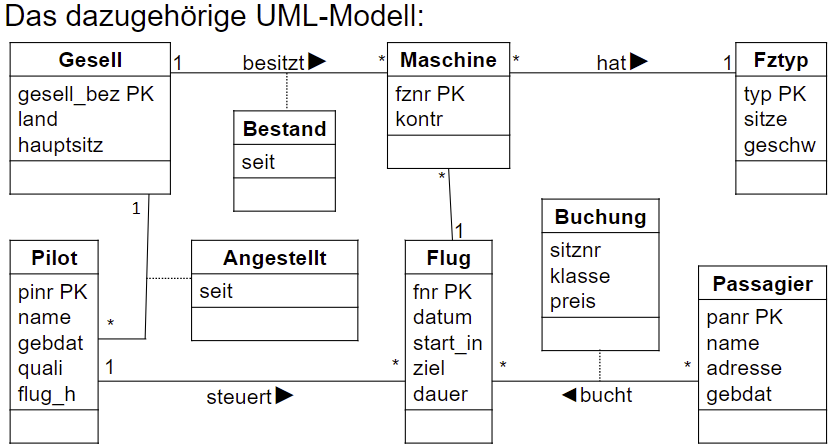
\includegraphics[scale=0.5]{20.png}
    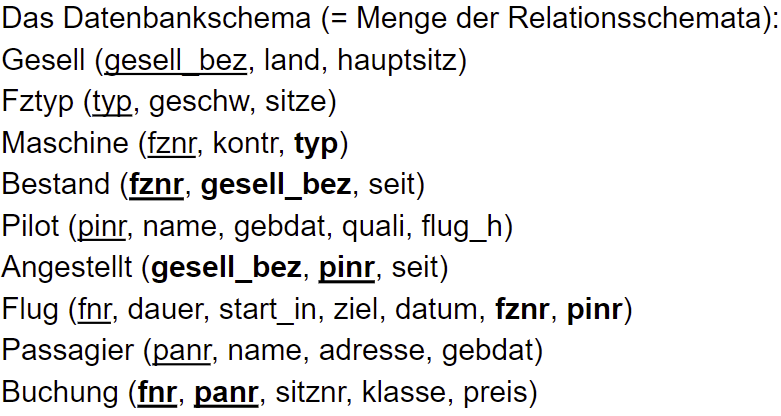
\includegraphics[scale=0.5]{21.png}
\end{center}


\noindent Formuliere die folgende Anfragen mit Hilfe der relationalen Algebra

\noindent a)Wie lauten die Namen (name) und Adressen (adresse) aller Passagiere? 所有乘客的姓名和地址是什么?

$\pi$[name, adresse] (Passagier)
\\
\\
\noindent b) Wie heißen die Flugkapitäne mit Qualität ,,Captain'' (pinr, name, flug\_h)? 质量为''机长”的飞行机长的名字是什么?

$\pi$[pinr, name, flug\_h] $\sigma$[quali= ''Captain''] (Pilot)
\\
\\
\noindent c) Welche verschiedenen Flugrouten existieren (start\_in, ziel, dauer)? 存在哪些不同的飞行路线?

$\pi$[start\_in, ziel, dauer] (Flug)
\\
\\
\noindent d) Von welchen Städten (start\_in) aus kann man nach ,,London'' oder ,,Berlin'' fliegen? 从哪些城市起飞可以飞到伦敦或柏林?

$\pi$[start\_in] $\sigma$[ziel = ''London'' $\vee$ ziel = ''Berlin''] (Flug)
\\
\\
\noindent e)Welche Piloten (name) sind nicht ,,Chefpilot'' und haben über 1500  Flugstunden (flug\_h) absolviert? 哪些飞行员不是Chefpilot,但拥有超过1500小时的飞行时长?

$\pi$[name, flug\_h] $\sigma$[quali $\neq$ ''Chefpilot'' $\wedge$flug\_h > 1500] (Pilot)

\noindent---------------------------------------------------------------------------------------------------------------------------------

\noindent Löse folgende Aufgaben unter Verwendung des Kreuzprodukts. 用叉积解决问题

\noindent Führe gegebenenfalls eine Umbenennung von Attributen / Relationen durch. 若有必要,可重命名
\\
\\
\noindent a)Welche Maschinen (fznr, typ, geschw) fliegen schneller als 870 km/h? 哪些机器速度超过870?

$\pi$[fznr, typ, geschw] $\sigma$[geschw> 870 $\wedge$ typ = mtyp] (($\rho$[mtyp $\leftarrow$ typ] (Maschine)) $\times$ Fztyp)
\\
\\
\noindent b) Welche Piloten (pinr, name) fliegen nach ,,Berlin''? 哪些飞行员飞向柏林?

$\pi$[pinr, name] $\sigma$[ziel = "Berlin" $\wedge$ pinr= f\_pinr] (($\rho$[f\_pinr $\leftarrow$ pinr] (Flug)) $\times$ Pilot)
\\
\\
\noindent c) Wann wurden die Maschinen von ,,AIR FRANCE'' das letzte Mal überprüft (fznr, kontr)? 叫,,AIR FRANCE''的机器上次检修是什么时候?

$\pi$[fznr, kontr] $\sigma$[gesell\_bez= ''AIR FRANCE'' $\wedge$ m\_fznr= fznr] (($\rho$[m\_fznr $\leftarrow$ fznr]   (Maschine)) $\times$ Bestand)
\\
\\
\noindent d) Welche Geschwindigkeiten fliegen die Maschinen von ,,AUSTRIAN AIRWAYS'' (fznr, typ, geschw)? AUSTRIAN AIRWAYS的哪些机器飞行速度都是啥? 

$\pi$[fznr, typ, geschw] $\sigma$[b\_fznr= fznr $\wedge$ mtyp= typ $\wedge$ gesell\_bez= "AUSTRIAN AIRWAYS"]  (($\rho$[mtyp $\leftarrow$ typ] (Maschine)) $\times$ ($\rho$[b\_fznr $\leftarrow$ fznr] (Bestand)) $\times$ Fztyp)
\\
\\
\noindent e) Von welchen Städten (start\_in) aus kann man sowohl nach ,,London'' als auch ,,Berlin'' fliegen?从哪些城市起飞,既可以到伦敦又可以到柏林?

$\pi$[start\_in] $\sigma$[ziel = "Berlin" $\wedge$ ziel2 = "London" $\wedge$ start\_in= start\_in2] (Flug $\times$ ($\rho$[fnr2,  datum2, start\_in2, ziel2, dauer2, fznr2, pinr2] (Flug)))

\section{Structured Query Language 结构化查询语言}

\subsection{概念}

\noindent SQL st eine Abfragesprache für relationale Datenbanken zum  Bearbeiten, Ändern oder Löschen und unabhängig vom DBMS. SQL是可编辑、更改或删除的关系数据库查询语言,并且独立于DBMS。

\noindent Relationale Algebra ist Grundlage für SQL. 关系代数是SQL的基础。

\noindent $\circ$ R A: \textcolor{red}{Projektion x} - \textcolor{orange}{Selektion x} \qquad - \textcolor[RGB]{84,139,84}{Tabellenname x,y}

\noindent $\circ$ SQL: \textcolor{red}{SELECT x} - \textcolor[RGB]{84,139,84}{FROM x,y} \qquad - \textcolor{orange}{WHERE x}

\textcolor{red}{Spalten(*)} - \textcolor[RGB]{84,139,84}{Quelle(Relation/Join)} \qquad - \textcolor{orange}{Bedingung(Filter)}
\\
\\
$\circ$ SQL kann erweiterte Begriffe benutzen: SQL可以使用扩展术语:

DISTINCT: gleiche Ergebnistupel werden entfernt. 差:删除相同的结果元组

AS:neu definierte Spalte oder Tabelle als Alias. 作为:新定义的列或表作为别名

GROUP-BY:Ausgabe unterschiedliche Werte einzeln oder als Ganzes. 单独或政体输出不同的值

HAVING :ähnlich zu WHERE, bezieht sich auf Ergebnisrelation. 类似于WHERE,是指定结果关系

ORDER BY:Attribute werden sortiert, Standard ist ASC, altn.: DESC. 属性被排列,标准是ASC,老的是DESC。

SUM,AVG, MIN, MAX:  Aufruf einer Funktion für Rückgabe Spalte. 调用返回列的函数。

NOW(): Funktion für Zeitbestimmung. 用于确定时间的函数

extract(): Funktion zur Wertezerlegung eines Eintrages. 用于条目的值分解的函数。

\subsection{SQL例子}

已知数据(见12页)

\noindent Formuliere einfache SQL-Anfragen für folgende Anforderungen.

\noindent a)Liste der Namen (name) und Adressen (adresse) aller Passagiere. 所有乘客的姓名和地址清单

SELECT name, adresse FROM passagier;
\\
\\
\noindent b) Liste aller Flugkapitäne ,,Captain'' (pinr, name, flug\_h). 所有机长的名单

SELECT pinr, name, flug\_h FROM pilot WHERE quali= 'Captain‘;
\\
\\
\noindent c) Liste der verschiedenen Flugrouten (start\_in, ziel, dauer). 不同飞行路线的列表

SELECT DISTINCT start\_in, ziel, dauer FROM flug;
\\
\\
\noindent d) Von welchen Städten (start\_in) kann man nach ,,London'' oder ,,Berlin'' fliegen?从哪个城市可以起飞可以到伦敦或柏林?

SELECT DISTINCT start\_in FROM flug WHERE ziel IN ('London', 'Berlin');
\\
\\
\noindent e) Welche Piloten (name) sind nicht ,,Chiefpilot'' und haben über 1500 Flugstunden (flug\_h) absolviert? 哪个飞行员不是Chiefpilot,但有超过1500小时飞行时长?

SELECT name, flug\_h FROM pilot WHERE quali!= 'Chiefpilot' AND flug\_h> 1500 ;
\\
\\
\noindent f) Liste aller Flüge (fnr, ziel) die nach ,,Berlin'', ,,London'', ,,Frankfurt'', ,,Paris'' oder ,,Koeln-Bonn'' gehen.能飞到柏林、伦敦、法兰克福、巴黎或科隆-波恩的飞机列表。

SELECT fnr, ziel FROM flug WHERE ziel IN ('Berlin', 'London', 'Frankfurt', 'Paris', 'Koeln-Bonn');
\\
\\
\noindent g) Liste aller Piloten, die ,,Captain'' oder ,,Chiefpilot'' sind(name, quali, flug\_h) und mehr als 1500  Flugstunden absolviert haben.飞行员列表,是Captain或Chiefpilot,有超过1500小时飞行时间。

SELECT name, quali, flug\_hFROM pilot WHERE quali IN ('Captain', 'Chiefpilot') AND flug\_h> 1500;

\noindent---------------------------------------------------------------------------------------------------------------------------------

Löse die folgenden Aufgaben zunächst durch Verwendung des Kreuzprodukts.
见Ü6 - 16

\noindent---------------------------------------------------------------------------------------------------------------------------------

\noindent a)Wie viele (anz) unterschiedliche Qualifikationen gibt es? 有多少种不同的资格?

SELECT count(DISTINCT quali) AS anz FROM pilot;
\\
\\
b) Welche Durchschnittsgeschwindigkeit (d\_geschw) weisen die Flugzeuge von ,,LUFTHANSA'' auf? LUFTHANSA的飞机的平均飞行速度是多少?

SELECT avg(geschw) AS d\_geschw FROM bestand NATURAL JOIN fztyp NATURAL JOIN maschine WHERE gesell\_bez= 'LUFTHANSA';
\\
\\
c) Wie viele Passagiere fliegen erster Klasse? 有多少乘客用一等舱?

SELECT count(panr) FROM buchung WHERE klasse = 1;
\\
\\
d) Wie viele Piloten (anz) mit der Qualifikation ,,Chiefpilot'' sind bei ,,AIR FRANCE'' beschäftigt? AIR FRANCE有多少Chiefpilot?

SELECT count(*) AS anz FROM pilot NATURAL JOIN angestellt WHERE quali= 'Chiefpilot' AND gesell\_bez= 'AIR FRANCE‘;
\\
\\
e) Wie viele Piloten (anz) gibt es für jede Qualifikation (quali)? 每种资格各有多少飞行员?

SELECT count(*) AS anz, quali FROM pilot GROUP BY quali;
\\
\\
f) Welche Piloten (pinr) sind für mehr als einen Flug (anz) eingesetzt? 哪些飞行员开1架以上的飞机?

SELECT pinr, count(*) AS anzFROM flug GROUP BY pinr HAVING count(*) > 1;
\\
\\
g) Welche Passagiere (panr) haben mehr als einen Flug (anz) gebucht? 哪些乘客订了1架以上的飞机?

SELECT panr, count(*) AS anz FROM buchung GROUP BY panr HAVING count(*) > 1;

\noindent---------------------------------------------------------------------------------------------------------------------------------

\noindent\textbf{UPDATE, INSERT INTO, DELETE FROM}

\noindent a)Der Pilot ,,Nico Oppermann'' ist ,,Captain'' geworden. 飞行员 Nico 变成了Captain

UPDATE pilot SET quali= 'Captain' WHERE name = 'Nico Oppermann';
\\
\\
b) Die Fluggesellschaft ,,BRITISH AIRWAYS'' hat am 2002-03-05 ein Flugzeug vom Typ ,,Airbus A319'' gekauft, das unter der internen Flugzeugnummer 274 erfasst wird. Die Kontrolle erfolgte am Kaufdatum.
''英国航空公司”航空公司于2002-03-05年购买了类型为''空中客车A319”的飞机,该飞机记录在内部飞机编号274上。 控制发生在购买之日。

INSERT INTO maschine(fznr, kontr, typ) VALUES (274, '2002-03-05', 'Airbus A319');

INSERT INTO bestand (fznr, gesell\_bez, seit)VALUES (274, 'BRITISH AIRWAYS‘, '2002-03-05');
\\
\\
c) Alle Flugzeuge von ,,AIR FRANCE'' wurden zuletzt am 2000-08-01 überprüft. 最后一次检查''法国航空”的飞机是在2000-08-01。

UPDATE maschine SET kontr= '2000-08-01' WHERE fznr IN (SELECT fznr FROM bestand 
WHERE gesell\_bez= 'AIR FRANCE');
\\
\\
d) Die Preise für alle Flüge in der 1. Klasse werden verdoppelt. 头等舱所有航班的价格都会加倍。

UPDATE buchung SET preis = preis * 2 WHERE klasse = 1;
\\
\\
e) Die ,,LUFTHANSA'' stellt einen neuen ,,Chiefpilot'' mit Namen ,,Albert Wutzler'' unter der Pilotennummer 293 ein. Dieser wurde am 23. August 1958 geboren und hat bisher 1695 Flugstunden absolviert. Er wird sofort eingestellt.
'' LUFTHANSA”正在以293号飞行员的名义雇用一个新的''首席飞行员”,名字叫'' Albert Wutzler”。 他出生于1958年8月23日,到目前为止已经完成了1695个小时的飞行。 他将被立即雇用。

INSERT INTO pilot(pinr, name, gebdat, quali, flug\_h) VALUES (293, 'Albert Wutzler','1958-08-23', 'Chiefpilot', 1695);

INSERT INTO angestellt (gesell\_bez, pinr, seit) VALUES ('LUFTHANSA', 293, now());
\\
\\
f) Die Buchung(en) für ,,Maria Langer'' soll(en) für den doppelten Preis in die erste Klasse umgewandelt werden.

UPDATE buchung SET preis = preis * 2, klasse = 1 WHERE panr IN (SELECT panr FROM passagier WHERE name = 'Maria Langer');
\\
\\
g) Der Flug mit Flugnummer 1 fällt aus. Dazugehörige Passagiere ohne weitere Buchungen werden ebenfalls gelöscht.
航班号1的航班已取消。 没有进一步预订的相关乘客也将被删除。

DELETE FROM buchung WHERE fnr= 1;

DELETE FROM flug WHERE fnr= 1;

DELETE FROM passagier WHERE panr NOT IN (SELECT panr FROM buchung);
\\
\\
h) Der Flugzeugtyp ,,Airbus A320'' wird ausgemustert. 飞机“空中客车A320”正在退役。

DELETE FROM buchung WHERE fnr IN (SELECT fnr FROM flug NATURAL JOIN maschine WHERE typ = 'Airbus A320');

DELETE FROM flug WHERE fznr IN (SELECT fznr FROM maschine WHERE typ = 'Airbus A320');

DELETE FROM bestand WHERE fznr IN (SELECT fznr FROM maschine WHERE typ = 'Airbus A320');

DELETE FROM maschine WHERE typ = 'Airbus A320';

DELETE FROM fztyp WHERE typ = 'Airbus A320';

DELETE FROM passagier WHERE panr NOT IN (SELECT panr FROM buchung);

\section{Normalisierung}

\subsection{1NF, 2NF, 3NF}

\noindent \textbf{1NF}: DieErste Normalform (1NF) ist dann gegeben, wenn alle Informationenin einer Tabelle \textcolor{orange}{atomar} vorliegen.
当表中的所有信息都是原子时,将给出第一个范式(1NF)。

d.h.: Jedes Attribut muss eindeutig aufgeschlüsselt sein ( z.B. Adresse).每个属性都必须明确列出(例如地址)
\\
\\
\textbf{2NF}: Eine Relation ist in der 2NF, wenn alle Nichtschlüsselattributwerte vom \textcolor{orange}{gesamten Primärschlüssel} abhängig sind. 当所有非关键属性值都依赖于整个主键时,则在2NF中存在一个关系。

d.h.: Alle Attribute müssen eine Beziehung zum gesamten Primärschlüssel zeigen (z.B. Rechnungsinformationen über KundenNr und dazugehörige Rechnungsnummer)
所有属性都必须显示与整个主键的关系(例如,有关客户编号的发票信息以及相关的发票编号)
\\
\\
\textbf{3NF}: Die 3NF ist das Ziel einer Normalisierung und dient der Performance, Redundanz und Flexibilität einer relationalen Datenbank. Sie besagt, dass alle Nichtschlüsselattribute \textcolor{orange}{voneinander unabhängig} sein müssen.
3NF是规范化的目标,可为关系数据库提供性能,冗余和灵活性。 它指出,所有非关键属性必须彼此独立。

d.h.: Funktionale Abhängigkeit der Attribute (z.B. Geburtsdatum und Alter). 属性的功能依赖性(例如出生日期和年龄)
\\
\\
Wichtig: Jede Normalform setzt die jeweils vorhergehende Normalform voraus.
重要提示:每个范式都需要以前的范式。

\subsection{例子}

\noindent\textbf{Bsp. 1}
\\
\\
Mit Hilfe der Relation Beleg (Gast\_ID, Zimmer\_Nr, Tag, Name, Vorname) werden Informationen über Gäste und ihre tägliche Zimmerbelegung gespeichert.
借助关系文档(来宾\_ID,房间\_Nr,日期,姓氏,名字),可以保存有关客人及其每日房间占用情况的信息。
\\
\\
a)Finde den oder die Schlüssel der Relation. 查找关系的一个或多个键。

Lösung 1: (Gast\_ID, Tag), Lösung 2: (Zimmer\_Nr, Tag)
\\
\\
b) Analysiere die Relation auf mögliche Anomalien. 分析该关系以查找可能的异常。

$\circ$ Einfüge-Anomalie: Ist ein Gast häufiger zu Besuch, müssen konstante Daten wie Name und Vorname wiederholt erfasst werden, was zu erhöhtem Arbeitsaufwand führt und eine potentielle Fehlerquelle ist, d.h. das Einfügen neuer Gäste ist nur in Verbindung mit einer Zimmerbelegung möglich.
插入异常:如果访客频繁访问,则必须重复记录诸如姓氏和名字之类的常量数据,这会增加工作量,并且是潜在的错误来源,即,仅在与房间占用有关的情况下才可以插入新访客。

$\circ$ Lösch-Anomalie: Mit dem Entfernen älterer Belegungen werden gleichzeitig die Informationen über Gäste eliminiert.
删除异常:由于删除了较早的入住,有关宾客的信息也将同时被消除。

$\circ$ Update-Anomalie: So oft ein Gast ein Zimmer belegt, wird sein Name (redundant) mitgeführt. Namensänderungen können zu widersprüchlichen Daten führen.
更新异常:当客人占用房间的频率很高时,他或她的名字会(多余地)随身携带。 名称更改可能导致数据冲突。
\\
\\
c) Überführe die Relation in die zweite Normalform. 将关系转换为第二范式。

Gast\_ID, Tag :

\indent\indent Aufteilung von Beleg, wegen Gast\_ID $\rightarrow$ (Name, Vorname):

\indent\indent\indent Gast (Gast\_ID, Name, Vorname)

\indent\indent\indent Beleg (Gast\_ID, Tag, Zimmer\_Nr)

Zimmer\_Nr, Tag :

\indent\indent (Gast\_ID, Zimmer\_Nr, Tag, Name, Vorname)
\\
\\
mit Lösung 2 Schlüssel wäre ursprüngliche Relation bereits in 2NF, da Aufteilung wegen (Zimmer\_Nr, Tag) $\rightarrow$ Gast\_ID $\rightarrow$ (Name, Vorname) erst bei 3NF nötig wäre.
使用解决方案2的键,原来的关系就已经在2NF中,因为由于(房间\_Nr,天)$ \rightarrow $客人\_ID $ \rightarrow $(姓,名)才需要划分,直到3NF

\noindent---------------------------------------------------------------------------------------------------------------------------------

\noindent\textbf{Bsp. 2} Ü9-A3

\noindent 已知:

依赖关系Relation R mit den funktionalen Abhängigkeiten(PNr $\rightarrow$ Name, ANr $\rightarrow$ Bez, PrNr $\rightarrow$ PrName,   PNr $\rightarrow$ ANr)

键Schlüssel(PNr, PrNr)

\begin{center}
    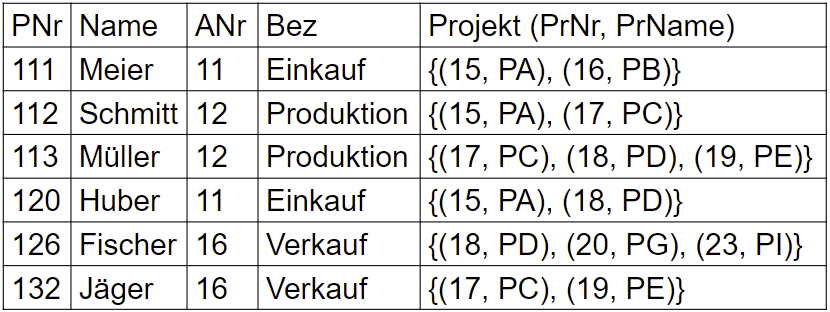
\includegraphics[scale=0.5]{22.png}
\end{center}

\noindent 求:其第三范式.in dritte Normalform
\\
\\
解:

\textbf{1.} 

先写出原式:R (\underline{PNr}, Name, ANr, Bez, Projekt (\underline{PrNr}, PrName))

判断出原式中嵌套了一个属性Projekt,因此并非第一范式1NF,而是NF$^2$(Non First Normal Form = keine atomaren Attribute).

\textbf{2.}

转化为1NF.

R0 (\underline{PNr}, Name, ANr, Bez, \underline{\textbf{PrNr}}, PrName)

\textbf{3.}

转化为2NF.

在R0中,判断\, 主键-非主键\, 之间是否有包含关系,若有,则提出来。

R1 (\underline{\textbf{PNr}}, \underline{\textbf{PrNr}})

R2 (\underline{PrNr}, PrName) $\leftarrow$ 可以看作是Projekt

R3 (\underline{PNr}, Name, ANr, Bez)

\textbf{4.}

转化为3NF.

判断R1, R2, R3中的\,非主键-非主键\,之间是否存在关系,若有,则提出来

可见R3中,ANr与Bez存在关系,则:

R31 (\underline{PNr}, Name, \textbf{ANr})

R32 (\underline{ANr}, Bez)

\textbf{$\Rightarrow$}

最终的3NF为:R1, R2, R31, R32

\section{Physische Datenorganisation}

\subsection{Bi-, B-Baum}

\noindent Binärer Suchbaum -Löschen durch Kopieren: 二进制搜索树 - 通过复制删除:

Jeder Knoten \textcolor{orange}{ohne Blatt} kann gelöscht werden, wenn dieser aber Blätter hat, müssen diese durch \textcolor{orange}{kopieren an eine andere Stelle} verschoben werden.
可以删除任何没有叶子(孩子)的节点。但如果有叶子,则必须通过复制他们移动到另一个位置。
\\
\\
B-Baum -Einfügen: 插入

In \textcolor{orange}{freie Blattknoten} können Elemente an die richtige Stelle eingefügt werden, wenn der Blattknoten voll ist, wird der \textcolor{orange}{Blattknoten aufgeteilt} und das Mittelelement in die den höheren Blattknote verschoben.
在自由叶子节点中,可以在正确的位置插入元素。当叶子节点已满时,叶子节点将拆分,中间元素移至较高的叶子节点。

Hinweis: Es kann durch Einfügen auch eine neue Wurzel entstehen.
注意:也可以通过插入来创建新的根。
\\
\\
B-Baum -Löschen: 删除

Löschen ist in B-Bäumen nur in Blattknoten möglich! Falls dies nicht vorliegt, muss durch Verschiebung des Elementes dies erreicht werden. Bei Unterschreitung/Überschreitung von Blattknoten kann dies wieder durch Verschiebung gelöst werden.
只能在叶子节点中删除!如果不是这种情况,则必须通过移动元素来实现。如果叶子节点低于/超过此值,则可以移动再次解决此问题。

Hinweis: In der Wurzel darf nicht gelöscht werden.注意:不得删除根!

\subsection{例子}

\noindent\textbf{Bsp. 1 Binärer Suchbaum 删除 löschen}

从图中删除13, 21, 39, 17。

思路:叶子节点直接删除。非叶子节点则复制过来其最大左孩子或最小右孩子,并在对应位置改好父子关系。

\begin{center}
    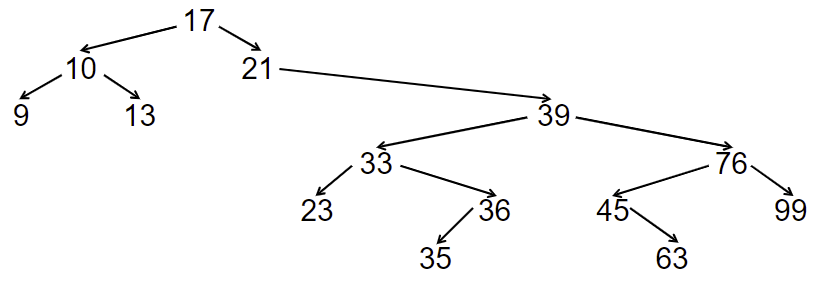
\includegraphics[scale=0.5]{23.png}

    删除13:
    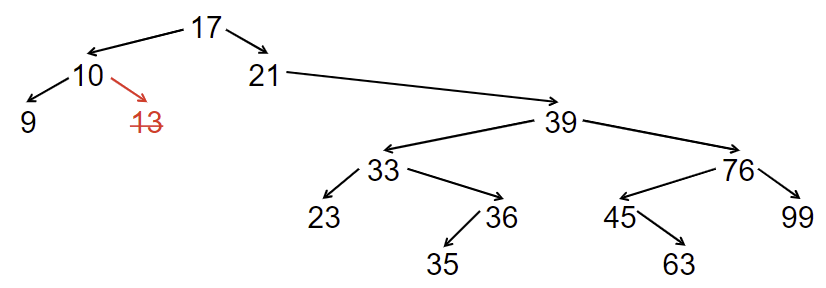
\includegraphics[scale=0.5]{24.png}

    删除21:
    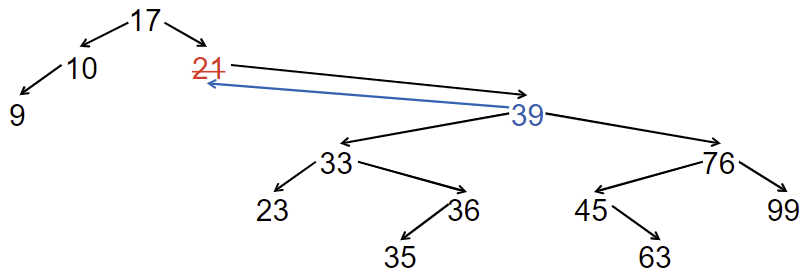
\includegraphics[scale=0.5]{25.png}

    删除39:
    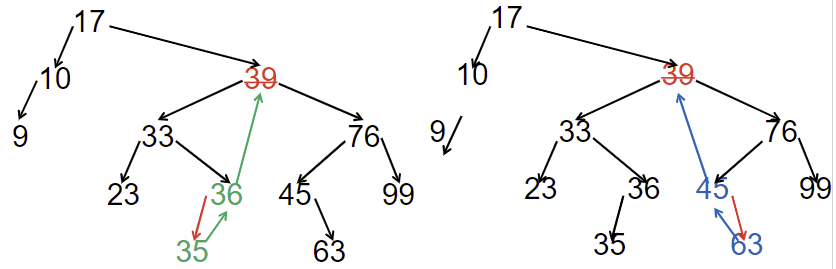
\includegraphics[scale=0.5]{26.png}

    删除17:
    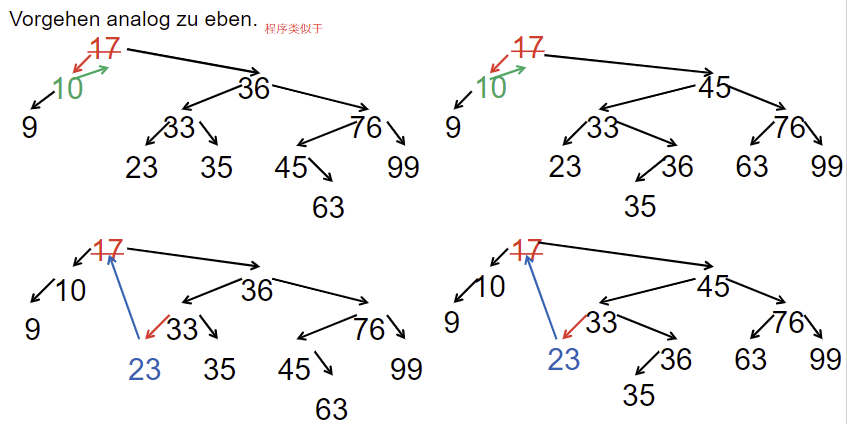
\includegraphics[scale=0.5]{27.png}

    结果:
    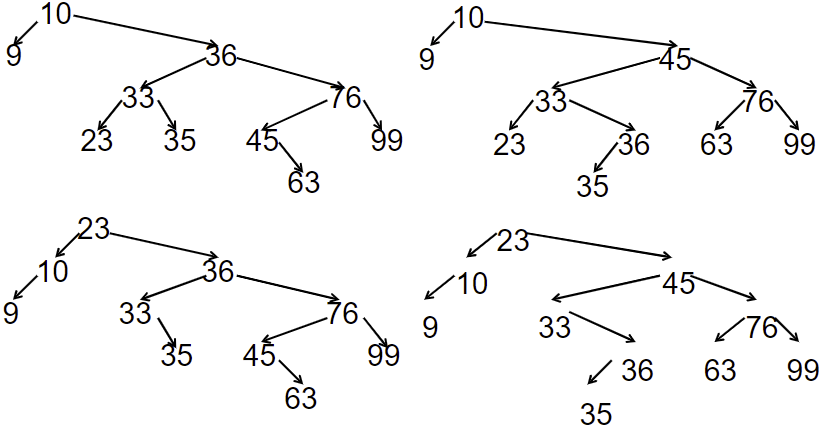
\includegraphics[scale=0.5]{28.png}
\end{center}

\noindent---------------------------------------------------------------------------------------------------------------------------------

\noindent\textbf{Bsp. 2 B-Baum 插入einfügen}

为以下高度为2阶为5(Höhe 2 und Ordnung 5)的B树插入33, 29,1。

思路:(33)若在叶子节点插入,直接插入即可。

(29)若相应的叶子节点已满,则需设置一个虚插入,形成如[22, 24, 26, 28, 29],然后将中间元素26移动至其父节点,左右两个拆为两个叶子节点。

(1)是进一步的推广。若已经是根结点,则直接再新建一个根结点。

\begin{center}
    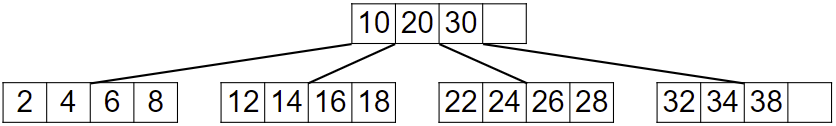
\includegraphics[scale=0.5]{29.png}

    插入33:
    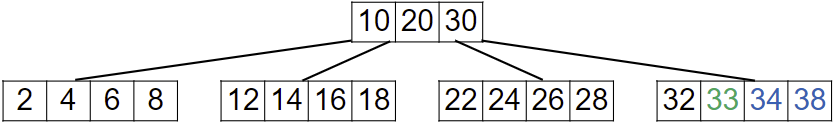
\includegraphics[scale=0.5]{30.png}

    插入29:
    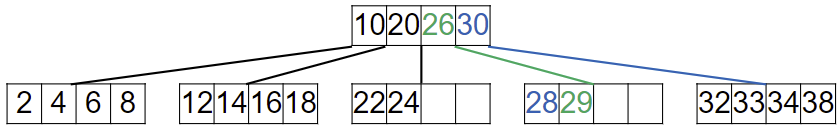
\includegraphics[scale=0.5]{31.png}

    插入1:
    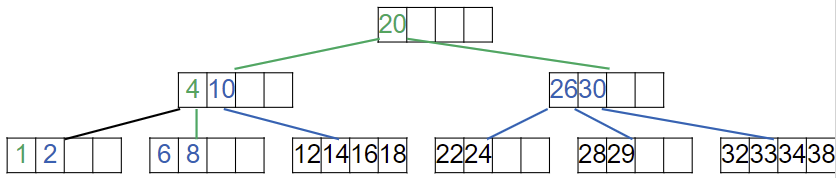
\includegraphics[scale=0.5]{32.png}

    结果:
    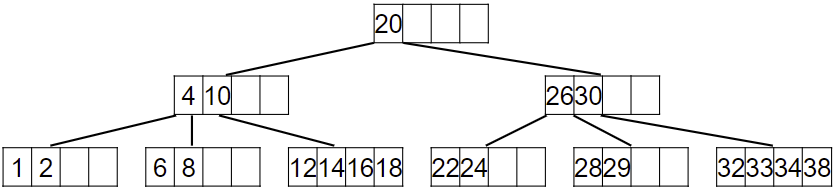
\includegraphics[scale=0.5]{33.png}
\end{center}

\noindent---------------------------------------------------------------------------------------------------------------------------------

\noindent\textbf{Bsp. 3 B-Baum  löschen}

删除48, 2

思路:

对于位于非叶子节点的元素,需要将其移动到叶子节点。并将另一个子节点中的下一个元素移动至其父节点。
随后需要判断节点(在上一步中将其元素移动至其父节点)是否符合最小填充量(minimale Füllmenge,似乎可以理解为最大填充量的一半,向下取整。)。
若不符合,则必须进行借元素或合并操作。

借元素操作:节点A存在直接相邻的兄弟节点B,且从B中借出1个元素后B仍符合最小填充量,则B中借出的元素上移(给父节点),父节点中的元素(介于A, B之间的元素)下移给A。

若节点B不符合最小填充量,则需合并:将父节点中的元素(介于A, B之间的元素)下移给A或B,然后合并AB即可。

\begin{center}
    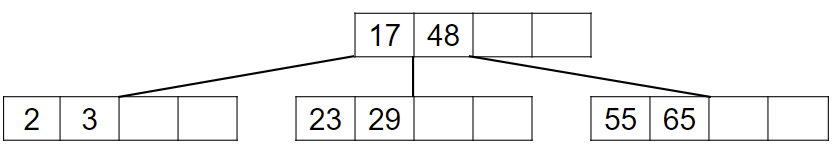
\includegraphics[scale=0.5]{34.png}

    删除48:
    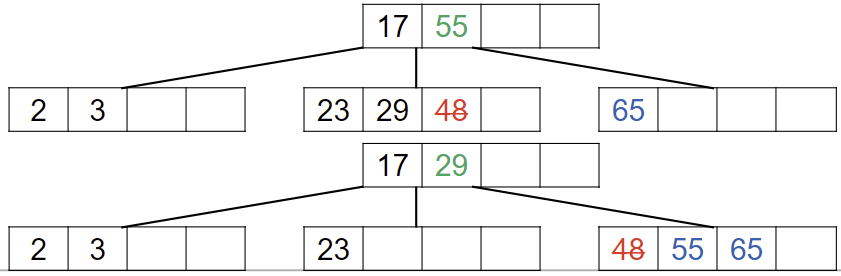
\includegraphics[scale=0.5]{35.png}

    合并:
    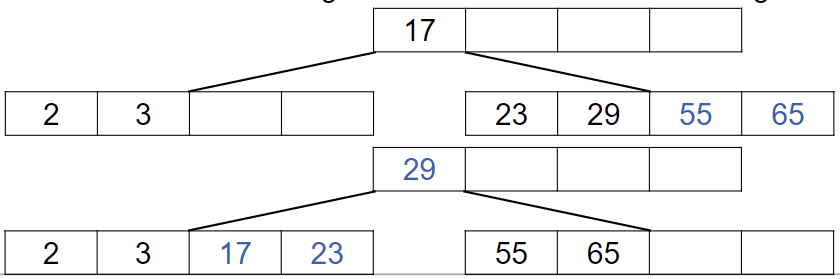
\includegraphics[scale=0.5]{36.png}

    删除2:
    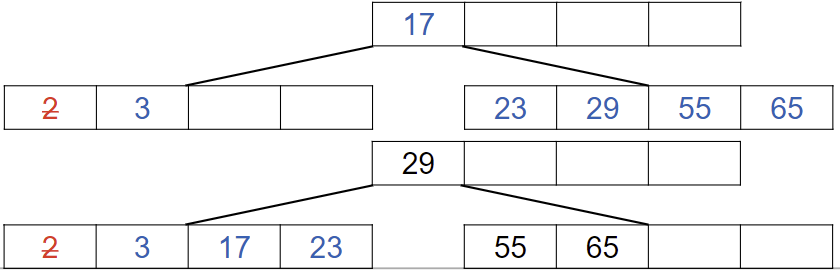
\includegraphics[scale=0.5]{37.png}

    结果:
    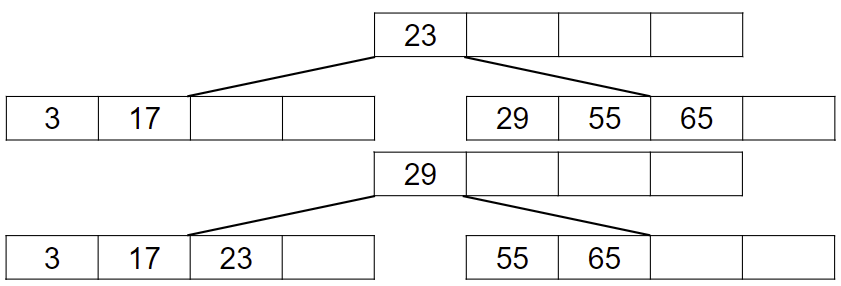
\includegraphics[scale=0.5]{38.png}
\end{center}

\section{Optimierung}

\subsection{定义:Optimierung von Datenbankabfragen}

\noindent $\circ$ Grundlage bildet immer die relationale Algebra mit ihren Operatoren
关系代数及其运算符始终构成基础
\\
\\
$\circ$ Bei jeder Optimierung werden die lesenden und schreibenden Zugriffe beachtet
每次优化都会考虑读写访问权限
\\
\\
$\circ$ Verschiedene Ansätze der Optimierung
不同的优化方法
\\
\\
$\circ$ Regelbasierte Optimierung wie Heuristik und kostenbasierte Optimierung durch optimale Joinreihenfolge
基于规则的优化,例如通过最佳联接顺序进行启发式和基于成本的优化
\\
\\
$\circ$ Beispiele: Reihenfolge der Joinsbeachten, äquivalente Ausdrücke umschreiben, Joinalgorithmen, Zugriffsart der Tabellen, JoinAusdrücke beachten
示例:观察联接的顺序,重写等效表达式,观察联接算法,表的访问类型,联接表达式
\\
\\
$\circ$ Anwendung: Selektionen aufteilen, Selektionen so weit unten wie möglich, Projektionen so weit unten wie möglich, Duplikateneleminierungentfernen, Kreuzprodukt zu Joinzusammenfassen, optimale Joinreihenfolge
应用程序:拆分选择,选择尽可能低,预测尽可能低,删除重复的删除项,将叉积组合为联接,最佳联接顺序

\subsection{例子}

\noindent\textbf{Bsp. 1}

\noindent 已知:

\begin{center}
    Operatorbaum 操作树
    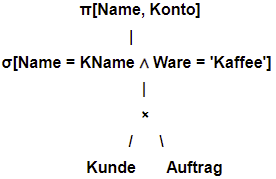
\includegraphics[scale=0.5]{39.png}
\end{center}

$\circ$ \textcolor{red}{Kunde} (Name, Kadr, Konto) umfasst \textcolor{red}{100} Tupel, wovon \textcolor{brown}{5} auf eine Seite passen

$\circ$ \textcolor{green}{Auftrag} (KName, Ware, Menge) umfasst \textcolor{green}{10.000} Tupel, wovon \textcolor[RGB]{84,139,84}{10} auf eine Seite passen  

$\circ$ \textcolor{violet}{50} Aufträge für die \textcolor{violet}{Ware Kaffee} existieren

$\circ$ \textcolor{brown}{50} Tupel (\textcolor{brown}{KName, Konto}) passen auf eine Seite

$\circ$ \textcolor{blue}{3} Tupel \textcolor{blue}{Kunde $\times$ Auftrag} passen auf eine Seite

$\circ$ Für jede Relation steht ein Puffer für genau eineSeite zur Verfügung. 每个关系都有一个恰好一侧的缓冲区。

$\circ$ es werden nur ganzeTupel auf einer Seite gespeichert. 页面上仅保存整个元组。

$\circ$ ein Seitenzugriff dauert lesend 1 msund schreibend 2 ms. 每页读1ms,写2ms。
\\
\\
\textbf{a)} Berechne die Zahl der Seitenzugriffe (Lesen, Schreiben) für die Auswertung desangegebenen Operatorbaums bei Zwischenspeicherung aller Zwischenergebnisse.
计算页面访问(读取,写入)的次数。

\textbf{1.} 

分析操作树:

$\sigma$操作就是查找操作,那么整棵树的意义为:查找买了咖啡(Ware='Kaffee')的顾客名Name和顾客账户Konto。

然后分析最内部的关系:KName $\wedge$ Ware 就是其叉乘,即:

R1:=Kunden $\times$ Auftrag

先算读取,则需要先列出所有顾客Kunden和订单Auftrag,并交叉对比(即乘积),其中读是按照页计算的。

Lesen: (\textcolor{red}{100}/\textcolor{brown}{5} * \textcolor{green}{10.000}/\textcolor[RGB]{84,139,84}{10}) = 20000 (次)

然后记录读取的结果,即写。即一共有多少页(Kunden $\times$ Auftrag)要写:

Schreiben: (\textcolor{red}{100} * \textcolor{green}{10.000}) / \textcolor{blue}{3} = 333334

\textbf{2.}

分析整个$\sigma$的情况:

R2:= $\sigma$[Name = KName $\wedge$ Ware = 'Kaffee'] R1  

则读取量就等于上一步的写入量:

Lesen: 333334

而符合条件的只有\textcolor{violet}{50}个,因为只存在\textcolor{violet}{50}个咖啡,那么这次的写入为:

Schreiben:\textcolor{violet}{50}/\textcolor{blue}{3} = 17

\textbf{3.}

分析剩下的$\pi$:

ERG:= $\pi$[Name, Konto] R2

因为上面计算出符合条件的数据只有17页,因此读=17:

Lesen: 17

而因为有\textcolor{violet}{50}个咖啡,那必然要写\textcolor{brown}{50}为一页的写入,则需要写入:

Schreiben: \textcolor{brown}{50}/\textcolor{violet}{50} = 1 页。

则有:

\textbf{Seitenzugriffe:} 20000 + 333334 + 333334 + 17 + 17 + 1 = 686703 次。
\\
\\
\textbf{b)}Optimiere den Operatorbaum und berechne die Seitenzugriffszahl erneut.
优化操作树并重新计算页面号Seitenzugriffszahl.

\begin{center}
    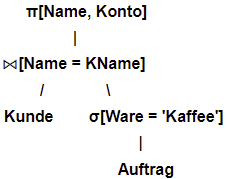
\includegraphics[scale=0.6]{40.png}
\end{center}

$\bowtie$ 的意思是Natural join (theta join).

\textbf{1.}

此时优化了Join的方法,使之在联合Kunden和Auftrag的时候就完成了筛选工作,节省了时间。

R1:= $\sigma$ [Ware = 'Kaffee'] Auftrag 

读,即在Auftrag中读取数据。

Lesen: \textcolor{green}{10.000}/\textcolor[RGB]{84,139,84}{10}=1000

写,仅记录\textcolor{violet}{50}条符合条件的数据,并形成一个临时的Auftrag':

Schreiben: \textcolor{violet}{50}/\textcolor[RGB]{84,139,84}{10} = 5

\textbf{2.}

R2:= Kunde $\bowtie$[Name=KName] R1

读,此时对比Auftrag'和Kunde,对比项是Name=KName:

Lesen: 5 * \textcolor{red}{100}/\textcolor{brown}{5} = 100

写:与a)同理:

Schreiben:\textcolor{violet}{50}/\textcolor{blue}{3} = 17

\textbf{3.}

ERG:= $\pi$[Name, Konto] R2

Lesen: 17

Schreiben: \textcolor{brown}{50}/\textcolor{violet}{50} = 1 

则有:

\textbf{Seitenzugriffe:} 1000 + 5 + 100 + 17 + 17 + 1 = 1140
\\
\\
\textbf{c)}Um welchen Faktor ist das optimierte Vorgehen schneller?
优化程序更快的因素是什么?

Dauer ursprünglich: a)的时长:(20000 + 333334 + 17) * 1ms + (333334 + 17 + 1) * 2ms = 1020055 ms

Dauer optimiert: b)的时长:(1000 + 100 + 17) * 1ms + (5 + 17 + 1) * 2ms = 1163 ms

Faktor schneller:提升倍率:1020055 / 1163 = 877

\section{Transaktionen}

\subsection{ACID-Prinzip}

\noindent$\circ$ Atomicity- Atomar 原子性-原子

$\circ$ ganz oder gar nicht 全有或全无

\noindent$\circ$ Consistency - Konsistent 一致性-一致

$\circ$ nach Ende der Transaktion konsistentes DBMS. DBMS在事物结束时保持一致

\noindent$\circ$ Isolation - Isoliert 隔离性-隔离

$\circ$ keine gegenseitige Beeinflussung 互不干扰

\noindent$\circ$ Durability- Dauerhaft 耐用性-永久

$\circ$ permanente Effekte 永久影响

\subsection{Ausführungsplan / Schedule}

\noindent$\circ$ Anordnung der Operationen von Transaktionen

\noindent$\circ$ Konflikterkennung

$\circ$ Operationen unterschiedlicher Transaktionen

$\circ$ Zugriff auf dasselbe Datenobjekt

$\circ$ darunter mindestens eine Schreiboperation

$\circ$ Erzeugung eines Log für jedes Datenbankobjekt hilfreich

\indent\indent$\circ$ zeitliche Folge von Datenbankoperationen auf einem Datenbankobjekt

\noindent$\circ$ Prüfung auf Konfliktserialisierbarkeit

\noindent$\rightarrow$ Präzedenzgraph (precedencegraph) erzeugen

$\circ$ Erzeugung eines Knotens für jede Transaktion

$\circ$ bei Konflikt Einfügen von Kante von älterer zu jüngerer Operation

$\circ$ Beschriftung der Kante mit Datenbankobjekt

$\circ$ wenn kein Zyklus existiert, ist Plan serialisierbar
\\
\\
\noindent$\circ$ 交易操作顺序

\noindent$\circ$ 冲突检测

$\circ$ 不同交易的操作

$\circ$ 访问相同的数据对象

$\circ$ 至少包括一个写操作

$\circ$ 为每个数据库对象生成日志很有帮助

\indent\indent$\circ$ 对数据库对象的数据库操作的时间顺序


\noindent$\circ$ 检查冲突的可序列化性

\noindent$\rightarrow$ 生成优先级图

$\circ$ 为每个事务生成一个节点

$\circ$ 如果存在冲突,请从较旧的操作到较新的操作插入一条边

$\circ$ 用数据库对象标记边缘

$\circ$ 如果不存在周期,则可以序列化计划

\subsection{例子}

\noindent\textbf{Bsp. 1}

\noindent Untersuchen Sie mit Hilfe eines Präzedenzgraphen, ob folgender Schedule S serialisierbarist!使用优先级图检查以下Schedule是否可以序列化.

\begin{center}
    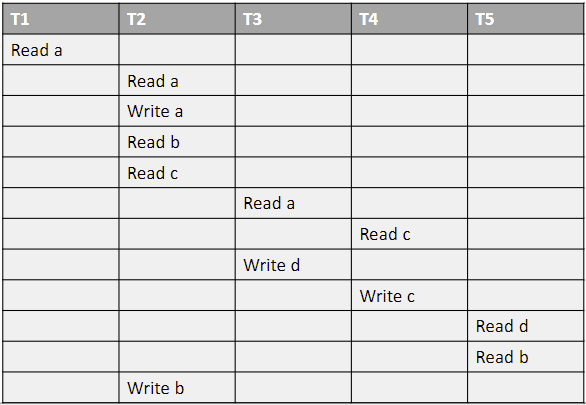
\includegraphics[scale=0.5]{41.png}
\end{center}

\noindent 解:

先写出流程图Log,即按照原图中的a, b, c, d作为标签,写出其访问顺序。

然后根据流程图画出优先级图。

\begin{center}
    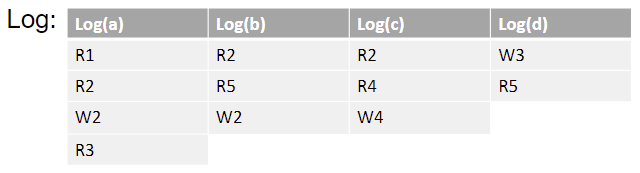
\includegraphics[scale=0.5]{42.png}
    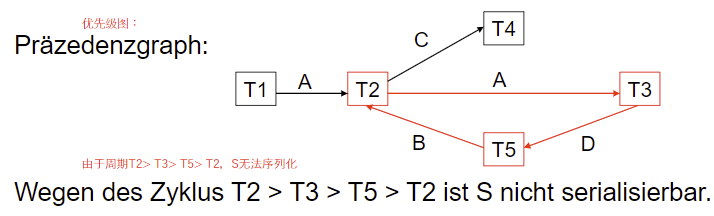
\includegraphics[scale=0.5]{43.png}
\end{center}

图中红色部分:见Log(b)中的顺序为R2$\rightarrow$R5$\rightarrow$W2,则需要画箭头从旧的T5指向新的T2。
画完整张图后,发现出现一个闭环,这意味着不能序列化。











\end{document}